\documentclass[12pt,border=4pt,multi]{article} % \documentclass[tikz,border=4pt,multi]{article}
\usepackage{lingmacros}
\usepackage{tree-dvips}
\usepackage{amssymb} % for mathbb{}
\usepackage[dvipsnames]{xcolor}
\usepackage{forest}
\usepackage{amsmath} % for matrices
\usepackage{xeCJK}
\usepackage{tikz}
\usepackage[arrowdel]{physics}
\usepackage{graphicx}
\usepackage{wrapfig}
\usepackage{listings}
\usepackage{pgfplots, pgfplotstable}
\usepackage{diagbox} % diagonal line in cell
\usepackage[usestackEOL]{stackengine}
\usepackage{multirow}
\graphicspath{{./img}} % specify the graphics path to be relative to the main .tex file, denoting the main .tex file directory as ./
\definecolor{orchid}{rgb}{0.7, 0.4, 1.1}

\begin{document}
\section*{Xi Liu, xl3504, lab 2 report}
Experiment 1:\\
assume 10 threads\\
x-axis = problem size\\
y-axis = (time of parallel part) / (total time from 
the time command)\\
/* from 0 to 100\% */\\
\begin{figure}[h!]
	\centering
	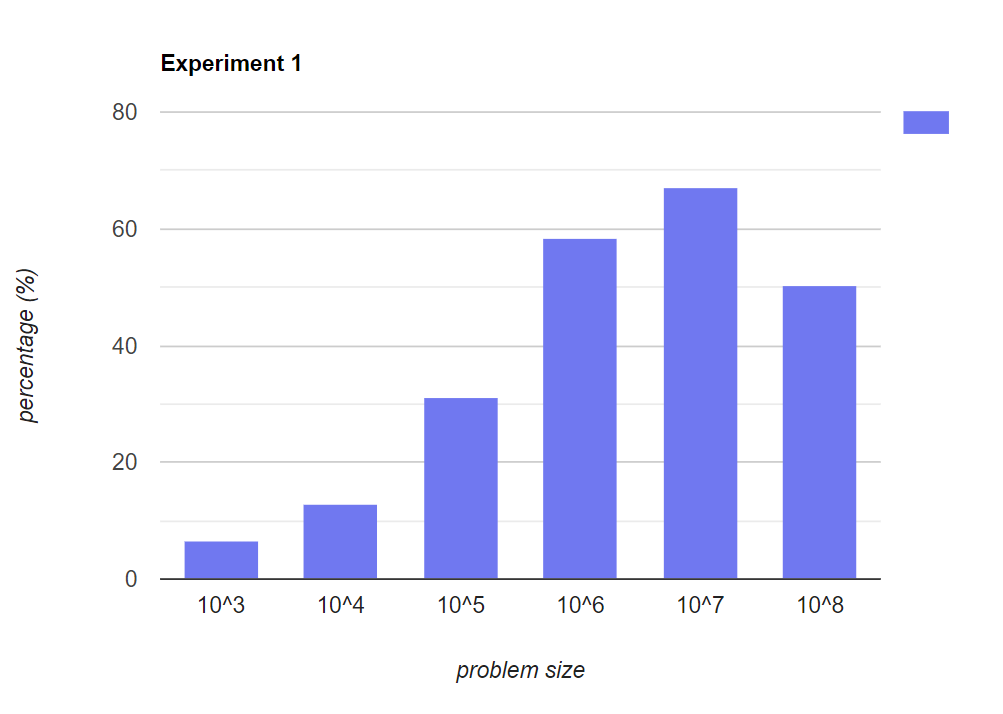
\includegraphics[width=1.1\textwidth, height=0.9\textwidth]{experiment 1} %img size
\end{figure}
\newpage
\noindent
Experiment 2\\
x-axis = number of threads\\
y-axis = speedup relative to sequential\\
input is a file of 1000,000 numbers and 50 bins\\
\begin{figure}[h!]
	\centering
	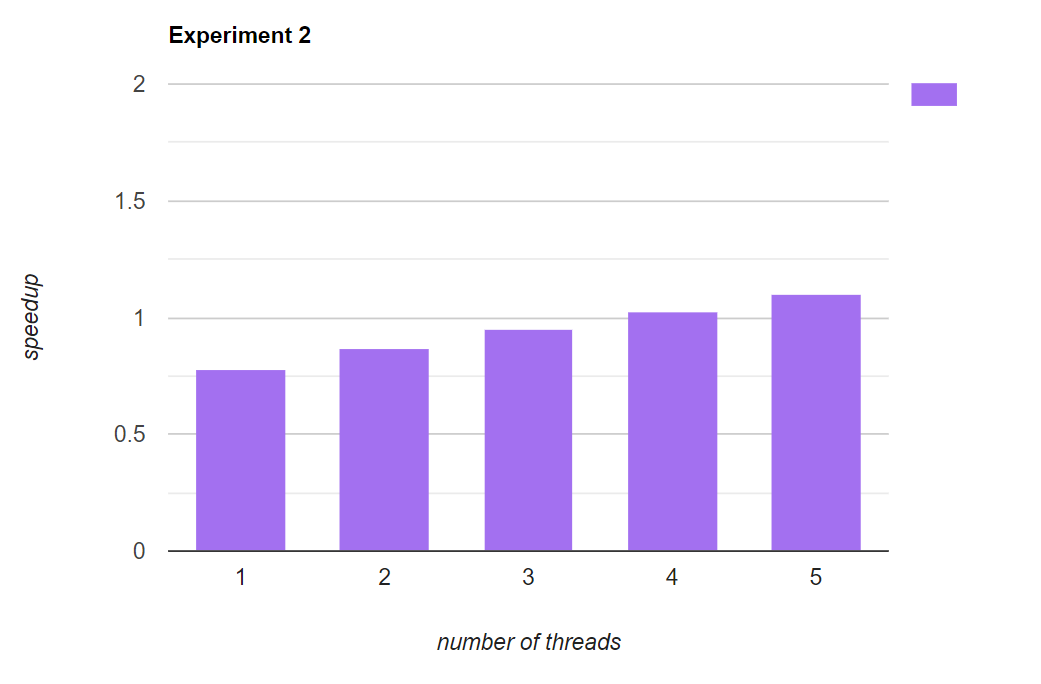
\includegraphics[width=1.1\textwidth, height=0.9\textwidth]{experiment 2} %img size
\end{figure}
\newpage
\noindent
Experiment 3\\
columns are problem size and rows are number of threads
{\Large
\begin{center}
\begin{tabular}{|c|c|c|c|c|c|} \hline
 & \textbf{1,000} & \textbf{10,000} & \textbf{100,000} & \textbf{1000,000} & \textbf{10,000,000}\\ \hline
\textbf{1} & 1 & 1 & 1 & 1 & 1\\ \hline
\textbf{2} & 0.598621 & 0.729739 & 0.623676 & 0.510030 & 0.506894\\ \hline
\textbf{3} & 0.452371 & 0.577546 & 0.409605 & 0.348475 & 0.345736\\ \hline
\textbf{4} & 0.294622 & 0.466245 & 0.292497 & 0.265548 & 0.261394\\ \hline
\textbf{5} & 0.174059 & 0.335924 & 0.262023 & 0.222585 & 0.214241\\ \hline
\end{tabular}
\end{center}
}
\leavevmode
\\
\\
\\
Analysis:\\
1.\\
the fraction of the time of sequential part (from the overall execution time) decreases as the problem size increases, since from experiment 1, the fraction of time of parallel part (from the overall execution time) increased as problem size increased\\
\\
2.\\
the speedup increases as the number of threads increases, both for the version of lab 1 and the version of this lab, since $speedup = T_{serial} / T_{parallel}$, and as number of threads increases, $T_{parallel}$ decreases until the number of threads reaches a threshold\\
\\
3.\\
the efficiency experiment produce the results I expected: let $p$ be the number of threads, then $efficiency = speedup / p = (T_{serial} / T_{parallel}) / p$, as the number of threads increases and reaches a threshold, $T_{parallel}$ would stop decrease (since there are more than enough threads and each thread is given too little work, and the overheads will increase when more threads need to access a critical section), but $p$ increases, so efficiency decreases\\
\end{document}